\documentclass[12pt, twoside]{article}
\usepackage[letterpaper, margin=1in, headsep=0.5in]{geometry}
\usepackage[english]{babel}
\usepackage[utf8]{inputenc}
\usepackage{amsmath}
\usepackage{amsfonts}
\usepackage{amssymb}
\usepackage{tikz}
\usetikzlibrary{quotes, angles}
\usepackage{graphicx}
\usepackage{enumitem}
\usepackage{multicol}

\newif\ifmeta
\metatrue %print standards and topics tags

\title{Regents Geometry}
\author{Chris Huson}
\date{September 2020}

\usepackage{fancyhdr}
\pagestyle{fancy}
\fancyhf{}
\renewcommand{\headrulewidth}{0pt} % disable the underline of the header
\raggedbottom


\fancyhead[LE]{\thepage}
\fancyhead[RO]{\thepage \\ Name: \hspace{4cm} \,\\}
\fancyhead[LO]{BECA / Dr. Huson / Geometry 08-Area+volume\\* pset ID: 140}

\begin{document}

\subsubsection*{8-6bDN-Solid-rotations}
\begin{enumerate}
\item Given $R(1,-5)$ and $S(5,7)$, find the length of $\overline{RS}$. Note: $l=\sqrt{(x_2-x_1)^2+(y_2-y_1)^2}$. \vspace{4cm}

\item On the graph, draw polygon ABCDEF with vertices A(2, 1), B(2, 4), C(4, 4), D(4, 8), E(8, 8), and F(8, 1). Find the perimeter and the area of the polygon.\\[1cm]
  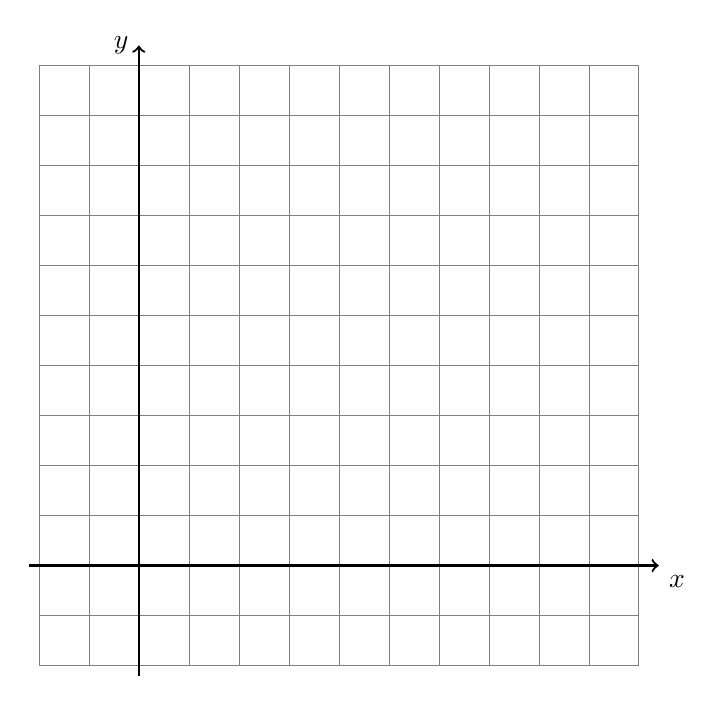
\begin{tikzpicture}[scale=.635]
    \draw [help lines] (-2,-2) grid (10,10);
    \draw [thick, ->] (-2.2,0) -- (10.4,0) node [below right] {$x$};
    \draw [thick, ->] (0,-2.2)--(0,10.4) node [left] {$y$};
  \end{tikzpicture}
  \vspace{1cm}
  
\item Find the area of a quarter circle with radius of 6 centimeters, expressed in terms of $\pi$.
  \begin{flushright}
   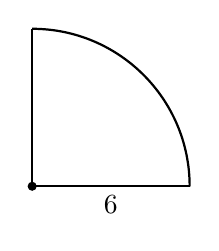
\begin{tikzpicture}[scale=1]
     %\draw [help lines] (-5,-1) grid (5,4);
     \draw [thick] (0,2)--(0,0)-- (2,0);
     %\draw [thick, ->] (0,-2.2)--(0,10.4) node [left] {$y$};
     \draw [thick] (2,0) arc (0:90:2);
     \draw [fill] (0,0) circle [radius=0.05];
     %\draw [fill] (2,0) circle [radius=0.05];
     \node at (1,0)[below]{6};
   \end{tikzpicture}
 \end{flushright} %\vspace{1cm}



\newpage
\subsubsection*{3-D Rotations \& Cross sections of solids}
\item %June 2019
    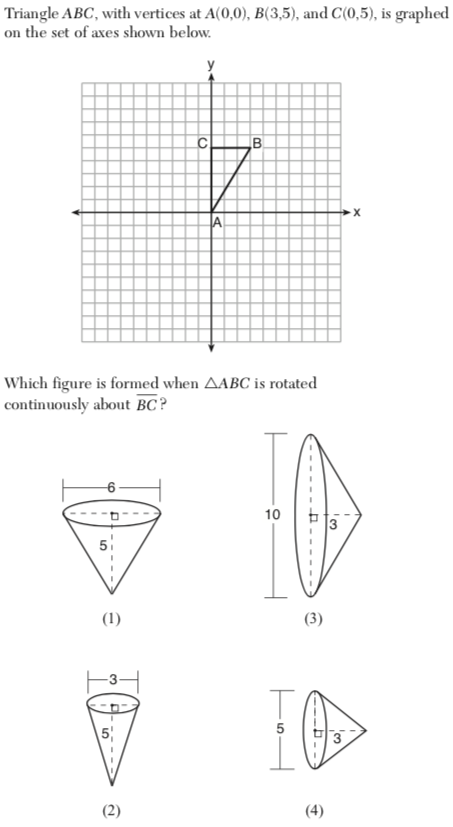
\includegraphics[scale=0.75]{triangle_3d_rotation_JN2018.png}

\newpage

\item %January 2018
  Circle $O$ is centered at the origin. In the diagram below, a quarter of circle $O$ is graphed.
    \begin{center}
      \begin{tikzpicture}[scale=0.6]
        %\draw [help lines] (-4,-4) grid (4,4);
        \draw [thick, <->] (-4,0) -- (4,0) node [below right] {$x$};
        \draw [thick, <->] (0,-3)--(0,3) node [left] {$y$};
        %\draw (0,0) circle [radius=2];
        \draw [thick] (-2,0) arc (180:270:2);
        \node at (0,0) [above right]{$O$};
      \end{tikzpicture}
      \end{center}
    Which three-dimensional figure is generated when the quarter circle is continuously rotated about the $y$-axis?
    \begin{multicols}{2}
      \begin{enumerate}
      \item cone
      \item sphere
      \item cylinder
      \item hemisphere
      \end{enumerate}
    \end{multicols}

\item A student has a rectangular postcard that he folds in half lengthwise. Next, he rotates it continuously about the folded edge. Which three dimensional object below is generated by this rotation?
    \begin{multicols}{2}
    \begin{enumerate}
      \item cone
      \item pyramid
      \item cylinder
      \item rectangular prism
    \end{enumerate}
    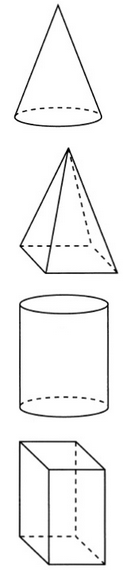
\includegraphics[scale=0.5]{solids.png}
    \end{multicols}

\newpage
\subsubsection*{Cross sections of solids} %2 problems in 6 exams
    
\item %January 2018
  A right hexagonal prism is shown below. A two-dimensional cross section that is perpendicular to the base is taken from the prism.
    \begin{center}
    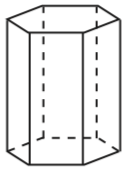
\includegraphics[scale=0.4]{hex-prism_JA2018.png}
    \end{center}
   Which figure describes the two-dimensional cross section?
    \begin{multicols}{2}
      \begin{enumerate}
        \item rectangle
        \item triangle
        \item pentagon
        \item hexagon
      \end{enumerate}
    \end{multicols}

\item  %August 2018
  A right cylinder is cut perpendicular to its base. The shape of the cross section is a
    \begin{multicols}{2}
      \begin{enumerate}
        \item circle
        \item cylinder
        \item rectangle
        \item triangular prism
      \end{enumerate}
    \end{multicols}
  
\item William is drawing pictures of cross sections of the right circular cone below.
    \begin{center}
      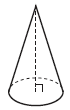
\includegraphics[]{cone.png}
    \end{center}
      Which drawing can \emph{not} be a cross section of a cone?
      \begin{multicols}{2}
      \begin{enumerate}
      \item square
      \item triangle
      \item parabola
      \item ellipse
      \end{enumerate}
      
\includegraphics[scale=0.7]{cone-sections.png}
    \end{multicols}

\end{enumerate}
\end{document}